\begin{figure}[!t]
\centering
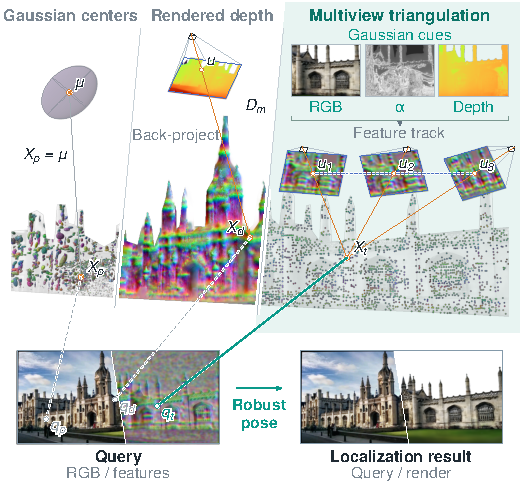
\includegraphics[width=\linewidth]{Fig1_geometry_to_localization.pdf}
\caption{From a Gaussian scene to a localization map. Gaussian centers and back-projected depth provide coordinate alternatives; our map triangulates multiview feature tracks. The lower panels show a query correspondence and alignment at the estimated Compact-map pose. Rendering visualizes the result and is not part of query localization.}
\label{fig:fig1}
\end{figure}
